\documentclass{article}

%%%%%%%%%%%%%%%%%%%%%%%% Importation de paquets %%%%%%%%%%%%%%%%%%%%
\usepackage{polyglossia}
\usepackage{graphics}
\usepackage{fontspec}
\usepackage{fancyhdr}
\usepackage{listings}
\usepackage{graphics}
\usepackage{fancyhdr}
\usepackage{vmargin}
\usepackage{epsfig}   
\usepackage{multicol}
\usepackage{multirow}
\usepackage{url,hyperref}

%%%%%%%%%%%%%%%%%%%%%%%% Format, langue, marges %%%%%%%%%%%%%%%%%%%%%%%%%%

\setdefaultlanguage{english}
\defaultfontfeatures{Mapping=tex-text,Scale=MatchLowercase}
\setmainfont{Linux Libertine O}
\setpapersize{A4}
\setmarginsrb   
{35mm}  % leftmargin
{20mm}  % topmargin
{35mm}  % rightmargin
{40mm}  % bottommargin
{14pt}  % headheight
{15mm}   % headsep
{20pt}  % footheight
{20mm}  % footskip

%%%%%%%%%%%%%%%%%%%%%%%% En-tete et pied de page %%%%%%%%%%%%%%%%%%%%%%%%%%
\pagestyle{fancy}
\fancyhf{}
\lhead{\scalebox{0.1}[0.1]{
\includegraphics{./Images/enseeiht}}}
\rhead{\scalebox{0.1}[0.1]{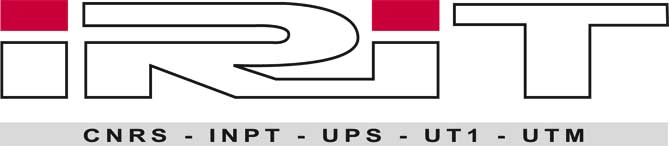
\includegraphics{./Images/irit}}
\lfoot{Three-dimensional modeling and printing}}
\rfoot{\bfseries \thepage}

\begin{document}

\bigskip
\bigskip
\bigskip
\bigskip
\bigskip
\bigskip
\bigskip
\bigskip

\begin{center}
\LARGE{Three-dimensional modelling and printing project :\\User documentation \\}
\bigskip
\bigskip\begin{tiny}
\end{tiny}
\Large{from January 23 to March 16, 2012}
\end{center}

\bigskip
\bigskip

\begin{center}
\large{
\textit{Vincent \textsc{Duvert} \\
Antoine \textsc{Lubineau} \\
Caroline \textsc{Naud} \\
James \textsc{Packer} \\
Florian \textsc{Ribon}} \\
\bigskip
INP-ENSEEIHT/IMA 
}
\end{center}

\bigskip
\bigskip

	This report summarizes the context, organization, work and outcomes within the project 3D modeling and printing project suggested by the VORTEX team of IRIT to some of the third-year students in the IMA department of ENSEEIHT.

\bigskip
\bigskip

\begin{figure}[!h]
\begin{center}
\scalebox{0.4}[0.4]{
\includegraphics{./Images/enseeiht}}
\end{center}
\end{figure}

\bigskip

\begin{center}
http://www.enseeiht.fr/fr/index.html \\
2 Rue Charles Camichel \\
31 071 TOULOUSE
\end{center}

\bigskip

\begin{figure}[!h]
\begin{center}
\scalebox{0.4}[0.4]{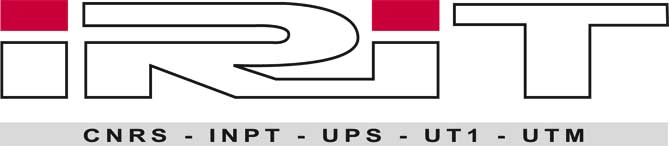
\includegraphics{./Images/irit}}
\end{center}
\end{figure}

\begin{center}
http://www.info@irit.fr\\
Université Paul Sabatier \\
118 Route de Narbonne \\
F-31062 TOULOUSE CEDEX 9
\end{center}

\thispagestyle{empty}

\newpage

\tableofcontents

\newpage

\section{Reminding of the global architecture of the application}


\begin{figure}[!h]
\begin{center}
\scalebox{0.4}[0.4]{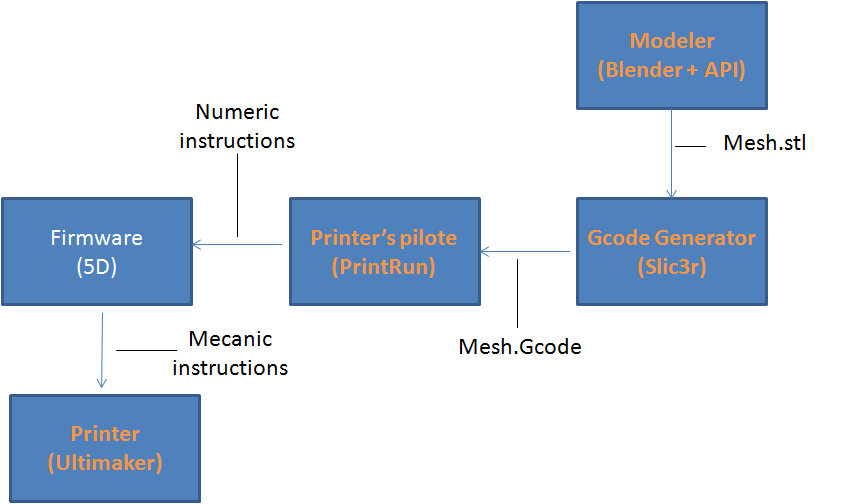
\includegraphics{./Images/ARD1}}
\end{center}
\end{figure}

\newpage

\section{The modelling part on Blender}

\subsection{Point on the graphic interface}

Mettre des Imprim écrans

\subsection{Obtaining a mesh}

\subsubsection{Loading a mesh for your personal files}

\subsubsection{Editing your own mesh}

\subsection{Verifying the quality of your mesh}

\subsection{Generating adequate supporting plans for your object}

\subsection{Choosing a good supporting plan}

\subsection{Saving your mesh}

\newpage

\section{The printing part}

\subsection{Preparing the Utimaker 3D printer}

It usually takes a bit of time to get a nice consistant extrusion at the beggining of the print, to avoid that put a few perimeters of skirt in Slic3r and push a bit on the filament during the first few seconds.
It is also a good idea to regularly check that the screw pushing on the filament stays nice and tight and that the roll of filament doesn't get caught and stop turning

\subsection{Generating the GCode on Slic3r}

First read \href{http://richrap.blogspot.com/2012/01/slic3r-is-nicer-part-1-settings-and.html}{this wiki} about the meaning of most the parameters.

And here are some useful values we found out worked fairly well in most cases :
Temperature : A good value is usually between 220 and 240. Lower and the plastic has difficulties sticking to the board at the beginning, higher and it might not cool down fast enough between layers. A high temperature also decreases the pressure the extruder has to apply
Extrusion multiplier : Because of difference in the way Slic3r and the arduino measure the length of filament to extrude (one measures it at the nozzle while to other does it at the motor) you have to multiply the theoritical value by a coefficient between 150 and 180.
Print speed : these five parameters depend mostly of the object's size. Indeed for most objects (30-30-60-60-60) are good value as they will insure a good quality and a good speed. However for small objects going too fast will not allow for enough time the layers to cool down and so the print will be less precise. The most 0.7 version of Slic"r corrects that bug by automatically slowing down when a layer is too small to cool down fast enough otherwise.
Layer height : The evident idea here is that a smaller layer height will make for a better quality. The values should be between 0.2 and 0.4 mm, however while 0.2 mm provides a very nice quality print it makes it longer and sometimes the plastic will bend more easily while cooling down.
Skirt : adding more loops before the actual print gives you a bit more time to make sur the extrusion is good.
Retraction : the values influence what the printer will do in case of a bridge (jumping from a position to another without extruding). Playing
There other settings we have tested that don't necessarily have an impact on the quality of the print but that are useful for other reasons.
Center : sets the center of the object you're going to print, the center of the plate is (100,100).
Copies along X/Y: very useful to do numerous copies of small objects.
Perimeters : can be played wth in the case of thin walled objects.
Infilling : the fastest to calculate is rectilinear but in some cases concentric is much more sensible (for instance, when most layer are homeomorphic to a circle.
\subsection{Sending the instructions to the printer with PrintRun}

\newpage

\section{Ending the work}

Comment fermer toutes les application après avoir sauvé une configuration \\
Parler de polir l'objet \\

\end{document}
